% =====================================================================
%  Wuhan (Yb) - Shanghai (Sr) optical-clock comparison:
%  tidal gravitational-redshift detection and fixed-coefficient
%  tidal corrections.
%
%  Submission draft (deliverable A).
%  Every numeric claim carries a "% src:" comment pointing at the
%  repository artifact it was read from.  Two numbers that remain
%  provisional (author list; the experiment-side per-segment counts,
%  which differ from this work's endpoint-trimmed counts) are marked
%  in place.
%
%  Compile:  pdflatex main.tex && bibtex main && pdflatex main.tex && pdflatex main.tex
% =====================================================================
\documentclass[11pt,a4paper]{article}

\usepackage[T1]{fontenc}
\usepackage[utf8]{inputenc}
\usepackage{amsmath}
\usepackage{amssymb}
\usepackage{graphicx}
\usepackage{booktabs}
\usepackage{geometry}
\usepackage[super,sort&compress]{natbib}
\usepackage[hidelinks]{hyperref}

% siunitx provides SI-unit and uncertainty typography.  This TeX Live 2023
% install does not ship it, so a compatible copy (v3.3.10, 2024-01-25) is
% installed in the user tree (~/texmf/tex/latex/siunitx).  Load it directly;
% do not pre-define \num/\qty fallbacks (they would clash with siunitx).
\usepackage{siunitx}
\sisetup{detect-all,separate-uncertainty=true}

\geometry{margin=2.5cm}

\newcommand{\Rdur}{R_{\mathrm{duration}}}
\newcommand{\Rwls}{R_{\mathrm{wls}}}
\newcommand{\dff}{\Delta f/f}
\newcommand{\dW}{\Delta W}
\newcommand{\Ffifteen}{F_{1550}}
\newcommand{\e}[1]{\times 10^{#1}}

\title{An inter-city optical clock network for precision metrology
and relativistic geodesy}

\author{%
  Haifeng Jiang%
  % NOTE: author list and affiliations are provisional.
  % Co-authors and institutional affiliations to be supplied by the
  % collaboration before submission; corresponding-author e-mail withheld
  % from this draft.
}
\date{}

\begin{document}
\maketitle

% =====================================================================
% SEGMENT-9-EXCLUDED VARIANT.  This file is an ADDITIVE sensitivity version
% of main.tex: it keeps the 17-segment manuscript untouched and re-renders
% the same text with segment 9 removed (16 segments).  Numbers marked
% "% seg9" below come from clock_ratio/statistical_methods_tidal_seg9_excluded.json
% and clock_ratio/correlation_reanalysis_seg9_independent.json.
% =====================================================================
\begin{abstract}
\sloppy
% =====================================================================
A redefinition of the SI second relies on optical frequency ratios that
different laboratories measure independently and that agree to within
$5\times10^{-18}$. Many optical clocks report self-evaluated uncertainties
meeting this level, but no comparison between clocks in different cities
has yet reached it. Here we close this gap with an inter-city,
cross-species clock network: an IAPMST ytterbium clock in Wuhan and a USTC
strontium clock in Shanghai, about \qty{700}{km} apart, are linked through a
\qty{1350}{km} phase-stabilised fibre and compared coherently for $58$\,days
(\qty{274}{h}, 16 segments with segment~9 excluded). Treating the tidal
gravitational-redshift term as an
uncertainty item, we obtain the Yb/Sr frequency ratio
$1.207\,507\,039\,343\,337\,720\,1(29)$, with a statistical uncertainty of
$0.88\times10^{-18}$ and a total uncertainty of $2\times10^{-18}$, whose
central value differs from the latest NIST--JILA result by less than
$5\times10^{-18}$. The same data show a tidal-template response in the
windowed beat series; fixed tidal-response scenarios change the
inter-segment scatter descriptively but are not used to correct the headline
ratio. The two clocks also read the time-varying
gravitational potential over the real \qty{700}{km} baseline, resolving a
tidal geopotential difference at centimetre-level equivalent height rather
than on a single campus. Such a network thus both supports the redefinition
of the SI second and senses the time-varying gravitational potential.
% seg9: 16-segment variant (segment 9 excluded). Headline ratio is the
%      UNCORRECTED centre 1.207...7201(29); the 0.88e-18 statistical term is
%      clock statistical noise only.
% src: clock_ratio/statistical_methods_tidal_seg9_excluded.json (raw scenario);
%      clock_ratio/correlation_reanalysis_seg9_independent.json;
%      clock/segment_analysis/batch_aggregate.csv (recomputed overlap-aware diagnostics).
% The European-network comparison is deliberately omitted: its statistical
% uncertainty is too large for a meaningful assertion of agreement, so the
% apparent concordance would be coincidental. Our own value may shift at the
% 1e-18 level once the full uncertainty evaluation is complete.
% NOTE: the total uncertainty is the quadrature sum of the Table 1 terms
% (2e-18). The clock-systematic terms are the published values; the tidal
% term is a theoretical bound. A full point-by-point systematics evaluation
% is still in progress and may refine the total.
\end{abstract}

% =====================================================================

\section{Introduction}
% =====================================================================
Optical clocks now measure frequency well enough to sense the
gravitational redshift over a height difference of a centimetre
\citep{mcgrew2018geodesy}, with self-evaluated fractional uncertainties
below $10^{-18}$ \citep{arnold2026lu, zhang2026ca} and two-clock
stabilities approaching $10^{-18}$ within an hour
\citep{oelker2019stability}, and their accuracy is driving two goals at
once: redefining the SI second on an optical transition and reading the
Earth's gravitational potential from clock comparisons
\citep{dimarcq2024roadmap, grotti2018geodesy}. Both goals, however,
depend on a capability that a single laboratory cannot provide. The best
clocks are not transportable, so their claimed accuracy can only be
confirmed by comparing them with one another over long distances. This
has motivated the concept of a clock \emph{network}, in which separate
clocks are linked into a single cooperative instrument
\citep{riehle2017networks, komar2014quantumnetwork}.

Fibre links have made such comparisons possible. Ultrastable light can
now be transferred over hundreds to thousands of kilometres with added
noise below the level of the clocks themselves
\citep{schioppo2022cavities, chen2026dissemination}, enabling inter-city
links \citep{lisdat2016network}, multi-species ratio measurements
\citep{beloy2021bacon}, and, most recently, a fibre network spanning
several countries \citep{pizzocaro2026european}; transportable clocks,
satellite links and free-space dissemination have extended comparisons
further \citep{laurent2015aces, lindvall2025coordinated,
shen2022freespace}. Beyond metrology, such
networks also probe fundamental physics, from gravitational waves
\citep{kolkowitz2016gw} to dark matter and topological defects
\citep{derevianko2014topological}. Yet the comparisons
reported so far fall short of what a redefined second requires. The
CCTF roadmap calls for optical frequency ratios measured independently
in different institutes and agreeing at the few-parts-in-$10^{18}$ level,
whose closure also validates the estimated uncertainties
\citep{dimarcq2024roadmap, riehle2015redefinition}: the only
cross-species ratio reported at this level was measured over a short
baseline between two clock laboratories in the same city
\citep{aeppli2026nist}, and the widest networks have not yet reached
$5\e{-18}$ \citep{lindvall2025coordinated}.

It therefore remains unclear whether two clocks of different species,
built at different institutions and separated by hundreds of kilometres
of fibre, can agree at the level a redefined second demands. Here we
show that they can. We link an ytterbium lattice clock at IAPMST in
Wuhan to a strontium lattice clock at USTC in Shanghai, about
\qty{700}{km} apart, through a \qty{1350}{km} phase-stabilised fibre, and
operate them coherently for $58$\,days. Treating the tidal
gravitational-redshift term as an uncertainty item, we obtain a Yb/Sr
ratio consistent with the existing determinations and observe a
tidal-template response that requires covariance-aware follow-up before a
formal detection claim.

% =====================================================================


% =====================================================================
\section{Results}
% =====================================================================

% =====================================================================
\subsection{Network and observation campaign}
\label{sec:network}
% =====================================================================

The experiment compares a Yb lattice clock at IAPMST in Wuhan
\citep{zhu2026yb} with a Sr lattice clock at USTC in Shanghai
\citep{jia2026sr}, two institutions and two clock
species about \qty{700}{km} apart. They are joined by a phase-stabilised
\qty{1550}{nm} fibre link of single-pass optical length $\approx1350$\,km,
deployed on paired strands within a single cable duct of a
telecommunications operator and organised as a cascade of relay stations,
each carrying a bidirectional erbium-doped fibre amplifier and a
fibre-noise-cancellation loop. Loop-back purification keeps the link
instability below the clock noise beyond \qty{\sim100}{s}
(Fig.~\ref{fig:setup}; Methods). The transfer architecture follows the
cascaded, bias-corrected optical-frequency-dissemination design
demonstrated on a \qty{2067}{km} field link \citep{chen2026dissemination}; the
present link is shorter, which relaxes the accumulated noise. The raw
observable is the out-of-loop beat note between the received carrier and
the local comb, sampled at \qty{1}{s}.

{\sloppy
Over a $58$-day campaign (2026-06-29 to 2026-08-26), 16 uninterrupted
segments (segment 9 excluded) yield $986\,416$ valid one-second samples
(\qty{274}{h}, a duty cycle of about $20\%$), gated by the simultaneous lock of both clocks
and the comb chain rather than by the link. The two clocks were
restarted independently between segments in the first campaign, so the
ratio centre provides a direct reproducibility check and shows no
measurable bias across restarts. The static geopotential difference,
$\dW = 280.042\pm0.085\ \mathrm{m^{2}/s^{2}}$ (Wuhan higher), is fixed
by first-order spirit levelling and applied as a constant correction
(Methods); its uncertainty enters the ratio budget as the $1\e{-18}$
static-redshift term (Table~\ref{tab:budget}). For the metrological
result we treat the time-varying tidal geopotential difference,
$\dW(t) = W_{\mathrm{WUHN}}(t) - W_{\mathrm{SHAN}}(t)$, as an
uncertainty item (Sec.~\ref{sec:tidal-theory}), taking its waveform
from a professional \qty{30}{s} series that combines solid-Earth tide and
ocean loading.
\par}
% src: docs/METHODOLOGY.md Sec. 0.1, docs/NOTATION.md Sec. 6, 8, 9;
% src: clock_ratio/ratio_17seg.csv; clock_ratio/tidal_correction/summary.json;
% src: paper/武汉-上海水准测量0930R1.docx; experiment-side manuscript (光钟比对论文 hj.docx, Sec. 2-3)

\begin{figure}[t]
  \centering
  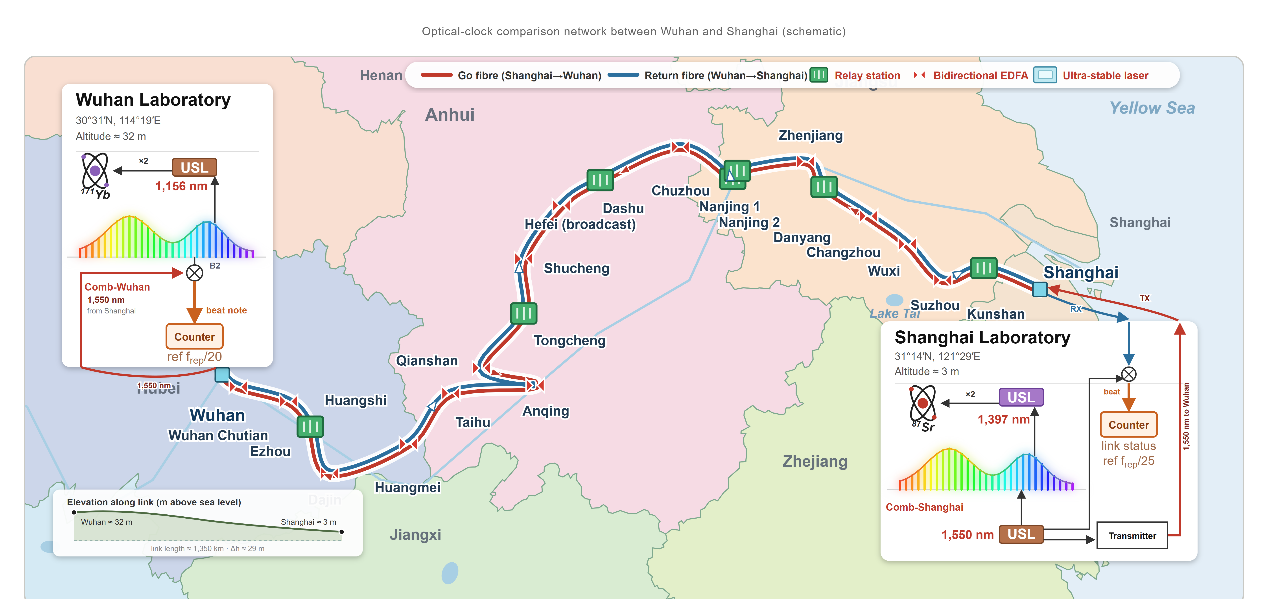
\includegraphics[width=0.95\linewidth]{figs/1.png}
  \caption{Experimental setup. The IAPMST Yb lattice clock in Wuhan and
  the USTC Sr lattice clock in Shanghai are linked by a phase-stabilised
  \qty{1550}{nm} fibre of single-pass optical length $\approx1350$\,km, with
  loop-back purification at each repeater; the out-of-loop beat note
  between the received carrier and the local comb is the raw observable.}
  \label{fig:setup}
\end{figure}

% =====================================================================


% ===== Clock-ratio determination =====

\subsection{Clock-ratio determination}
\label{sec:methods}

Combining the per-segment ratios with a random-effect model gives the
uncorrected Yb/Sr frequency ratio
\begin{equation}
  \mathrm{Yb/Sr} = 1.207\,507\,039\,343\,337\,720\,1(29),
  \label{eq:result-bayes}
\end{equation}
% seg9: 16-segment value from clock_ratio/statistical_methods_tidal_seg9_excluded.json (raw)
with a Bayesian statistical uncertainty of $0.88\e{-18}$ from the clock
statistical noise alone. The parenthetical $(29)$ is the display
precision of the value string, not the statistical term. The alternative
tidal-correction scenarios shift the centre by only a few
$10^{-19}$ relative to the experiment-side tidal-corrected value, and an independent
re-derivation from the raw beat files reproduces the per-segment ratios
exactly (Methods).

Table~\ref{tab:budget} lists the uncertainty terms. The Yb-clock
evaluation \citep{zhu2026yb} ($1.1\e{-18}$) and the static gravitational
redshift ($1\e{-18}$) dominate; the Sr-clock term \citep{jia2026sr} is
$9.2\e{-19}$, the fibre and comb terms are each below $1\e{-19}$, and the
tidal term is carried as an uncertainty item of $<5\e{-19}$, the size of
the theoretical compensation. Combined in quadrature these terms give a
total fractional uncertainty of $2\e{-18}$. The clock-systematic terms
are the published evaluations of the two clocks \citep{zhu2026yb,
jia2026sr}, and the tidal-model contribution is a theoretical bound; a
full point-by-point systematics evaluation remains in progress.
% src: experiment-side PDF (clock/潮汐修正后的比值计算.pdf) Sec. 5.4-5.6;
% src: clock/clock_tidal_shift.csv (tidal compensation magnitude < 5e-19);
% src: zhu2026yb (Yb clock: total systematic 1.3e-18); jia2026sr (Sr clock: <1e-18)

\begin{table}[t]
  \centering
  \caption{Corrections and uncertainty terms for the Yb/Sr ratio
  (fractional frequency units). ``Correction'' is the applied shift to
  the central value; ``Uncertainty'' is the term's contribution to the
  budget, combined in quadrature. The tidal term is carried as an
  uncertainty item (no correction applied; Sec.~\ref{sec:tidal-theory}).
  The total is the quadrature sum of the listed terms.}
  \label{tab:budget}
  \begin{tabular}{lcc}
    \toprule
    Source & Correction & Uncertainty \\
    \midrule
    Sr-clock systematic      & $9.2\e{-19}$ & $9.2\e{-19}$ \\
    Yb-clock systematic      & $1.1\e{-18}$ & $1.1\e{-18}$ \\
    Static gravitational redshift & $-3.1\e{-15}$ & $1\e{-18}$ \\
    Fibre transfer           & --- & $<1\e{-19}$ \\
    Comb transfer            & --- & $<1\e{-19}$ \\
    Statistical (Bayesian)   & --- & $0.88\e{-18}$ \\
    Tidal term (item)        & --- & $<5\e{-19}$ \\
    \midrule
    Total                    & --- & $2\e{-18}$ \\
    \bottomrule
  \end{tabular}
  % src: experiment-side PDF (clock/潮汐修正后的比值计算.pdf) Sec. 5.4-5.6;
  % src: clock/clock_tidal_shift.csv (tidal compensation magnitude < 5e-19);
  % src: delta_g = -3.1159e-15 (static gravitational correction, clock/shared.py)
\end{table}


Figure~\ref{fig:ratio} shows the clock-ratio data behind
Eq.~\eqref{eq:result-bayes}: the 16 per-segment ratios $R_i$ and the
segment-to-segment stability. In terms of the deviations
$y_i = R_i/R_{\mathrm{seg1}} - 1$, the duration-weighted mean is
$-0.639\e{-18}$ (arithmetic mean $-0.292\e{-18}$) and the segment-to-segment
scatter is $\sigma(y_i) = 2.58\e{-18}$.
% seg9: 16-segment values (segment 9 excluded) from ratio_17seg.csv
%      (duration-weighted mean -0.63866, arithmetic mean -0.2923, sigma 2.5805)

\begin{figure}[t]
  \centering
  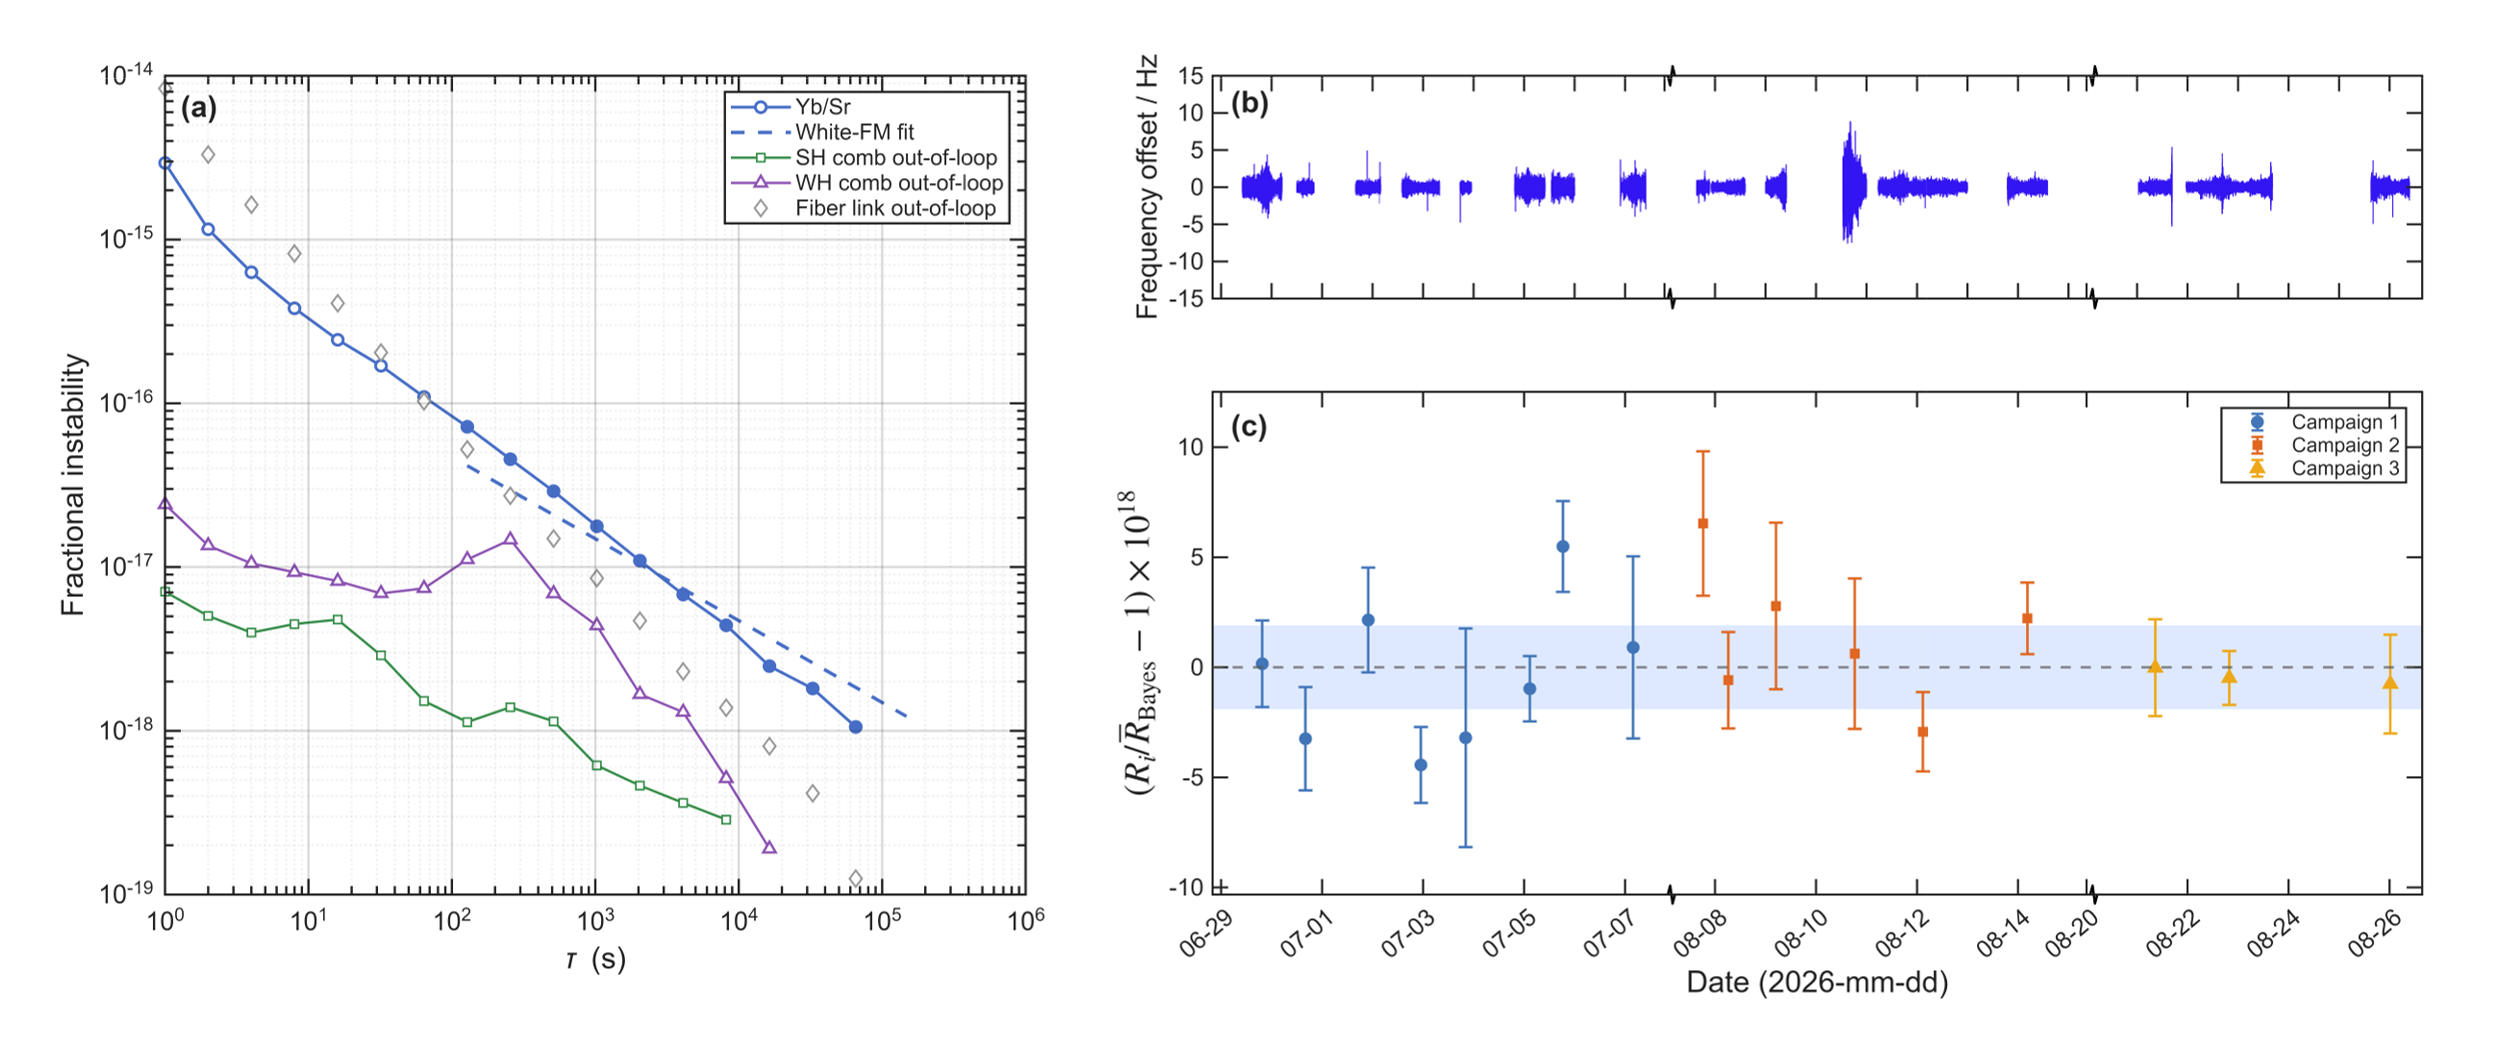
\includegraphics[width=0.95\linewidth]{figs/2.png}
  \caption{Clock-ratio data. The segment stability and the 16 per-segment
  Yb/Sr ratios $R_i$ (segment 9 excluded) give the deviation
  $y_i = R_i/R_{\mathrm{seg1}} - 1$
  whose duration-weighted mean is $-0.639\e{-18}$ and whose
  segment-to-segment scatter is $\sigma(y_i) = 2.58\e{-18}$.}
  \label{fig:ratio}
\end{figure}

% =====================================================================


% ===== Tidal detection =====

\subsection{Tidal gravitational-redshift detection}
\label{sec:detection}

The tide modulates the comparison frequency through the gravitational
redshift, $\dff/f = \dW(t)/c^{2}$, with a segment-averaged rms amplitude
of $3.90\e{-18}$ (median; range $2.00$--$6.56\e{-18}$ across the 16
segments).
% seg9: 16-segment tide_rms/F_1550 (segment 9 excluded); median 3.895e-18,
%      min 1.997e-18, max 6.562e-18

After both the beat and a tidal template are passed through a
\qty{1200}{s} triangular window and demeaned, each segment is fitted with
$A = \sum(\mathrm{tide}\cdot\mathrm{beat})/\sum\mathrm{tide}^{2}$. The
template is normalised to the \qty{1550}{nm} transfer frequency
$\Ffifteen=\qty{193.40}{THz}$, not to the ratio-conversion coefficient
$1/\mathrm{COEF}\approx\qty{233.53}{THz}$; the two differ by the Yb/Sr factor
$1.2075$, so the choice of reference sets the amplitude scale and must be
accounted for before comparing $A$ with other tidal analyses (Methods). A
single segment reaches only $\mathrm{SNR}\approx0.28$. The 600-s-step
windows overlap, so they cannot be used as independent samples for the
historical p values or ``sign-agnostic Stouffer'' score. The amplitude point
estimate uses all windows; its uncertainty and per-segment correlation are
now evaluated from non-overlapping 1200-s windows, pending a full
correlated-noise model. The historical fitted amplitude was approximately
\begin{equation}
  A \approx -0.54,
  \label{eq:Afit}
\end{equation}
% src: clock/segment_analysis/batch_aggregate.csv (must be regenerated after
%      the non-overlapping-window and validated-interpolation changes).
and is consistent with a response of roughly half the theoretical magnitude.
It is not used as a calibrated correction. At the segment-mean level, the ratio deviation $y_i$ is
positively correlated with the tidal shift $\dff$ (Pearson $r=+0.429$,
$p=0.098$).
% seg9: 16-segment correlation from correlation_reanalysis_seg9_independent.json
%      (pearson_r=0.428662, pearson_p=0.097585)

\begin{figure}[t]
  \centering
  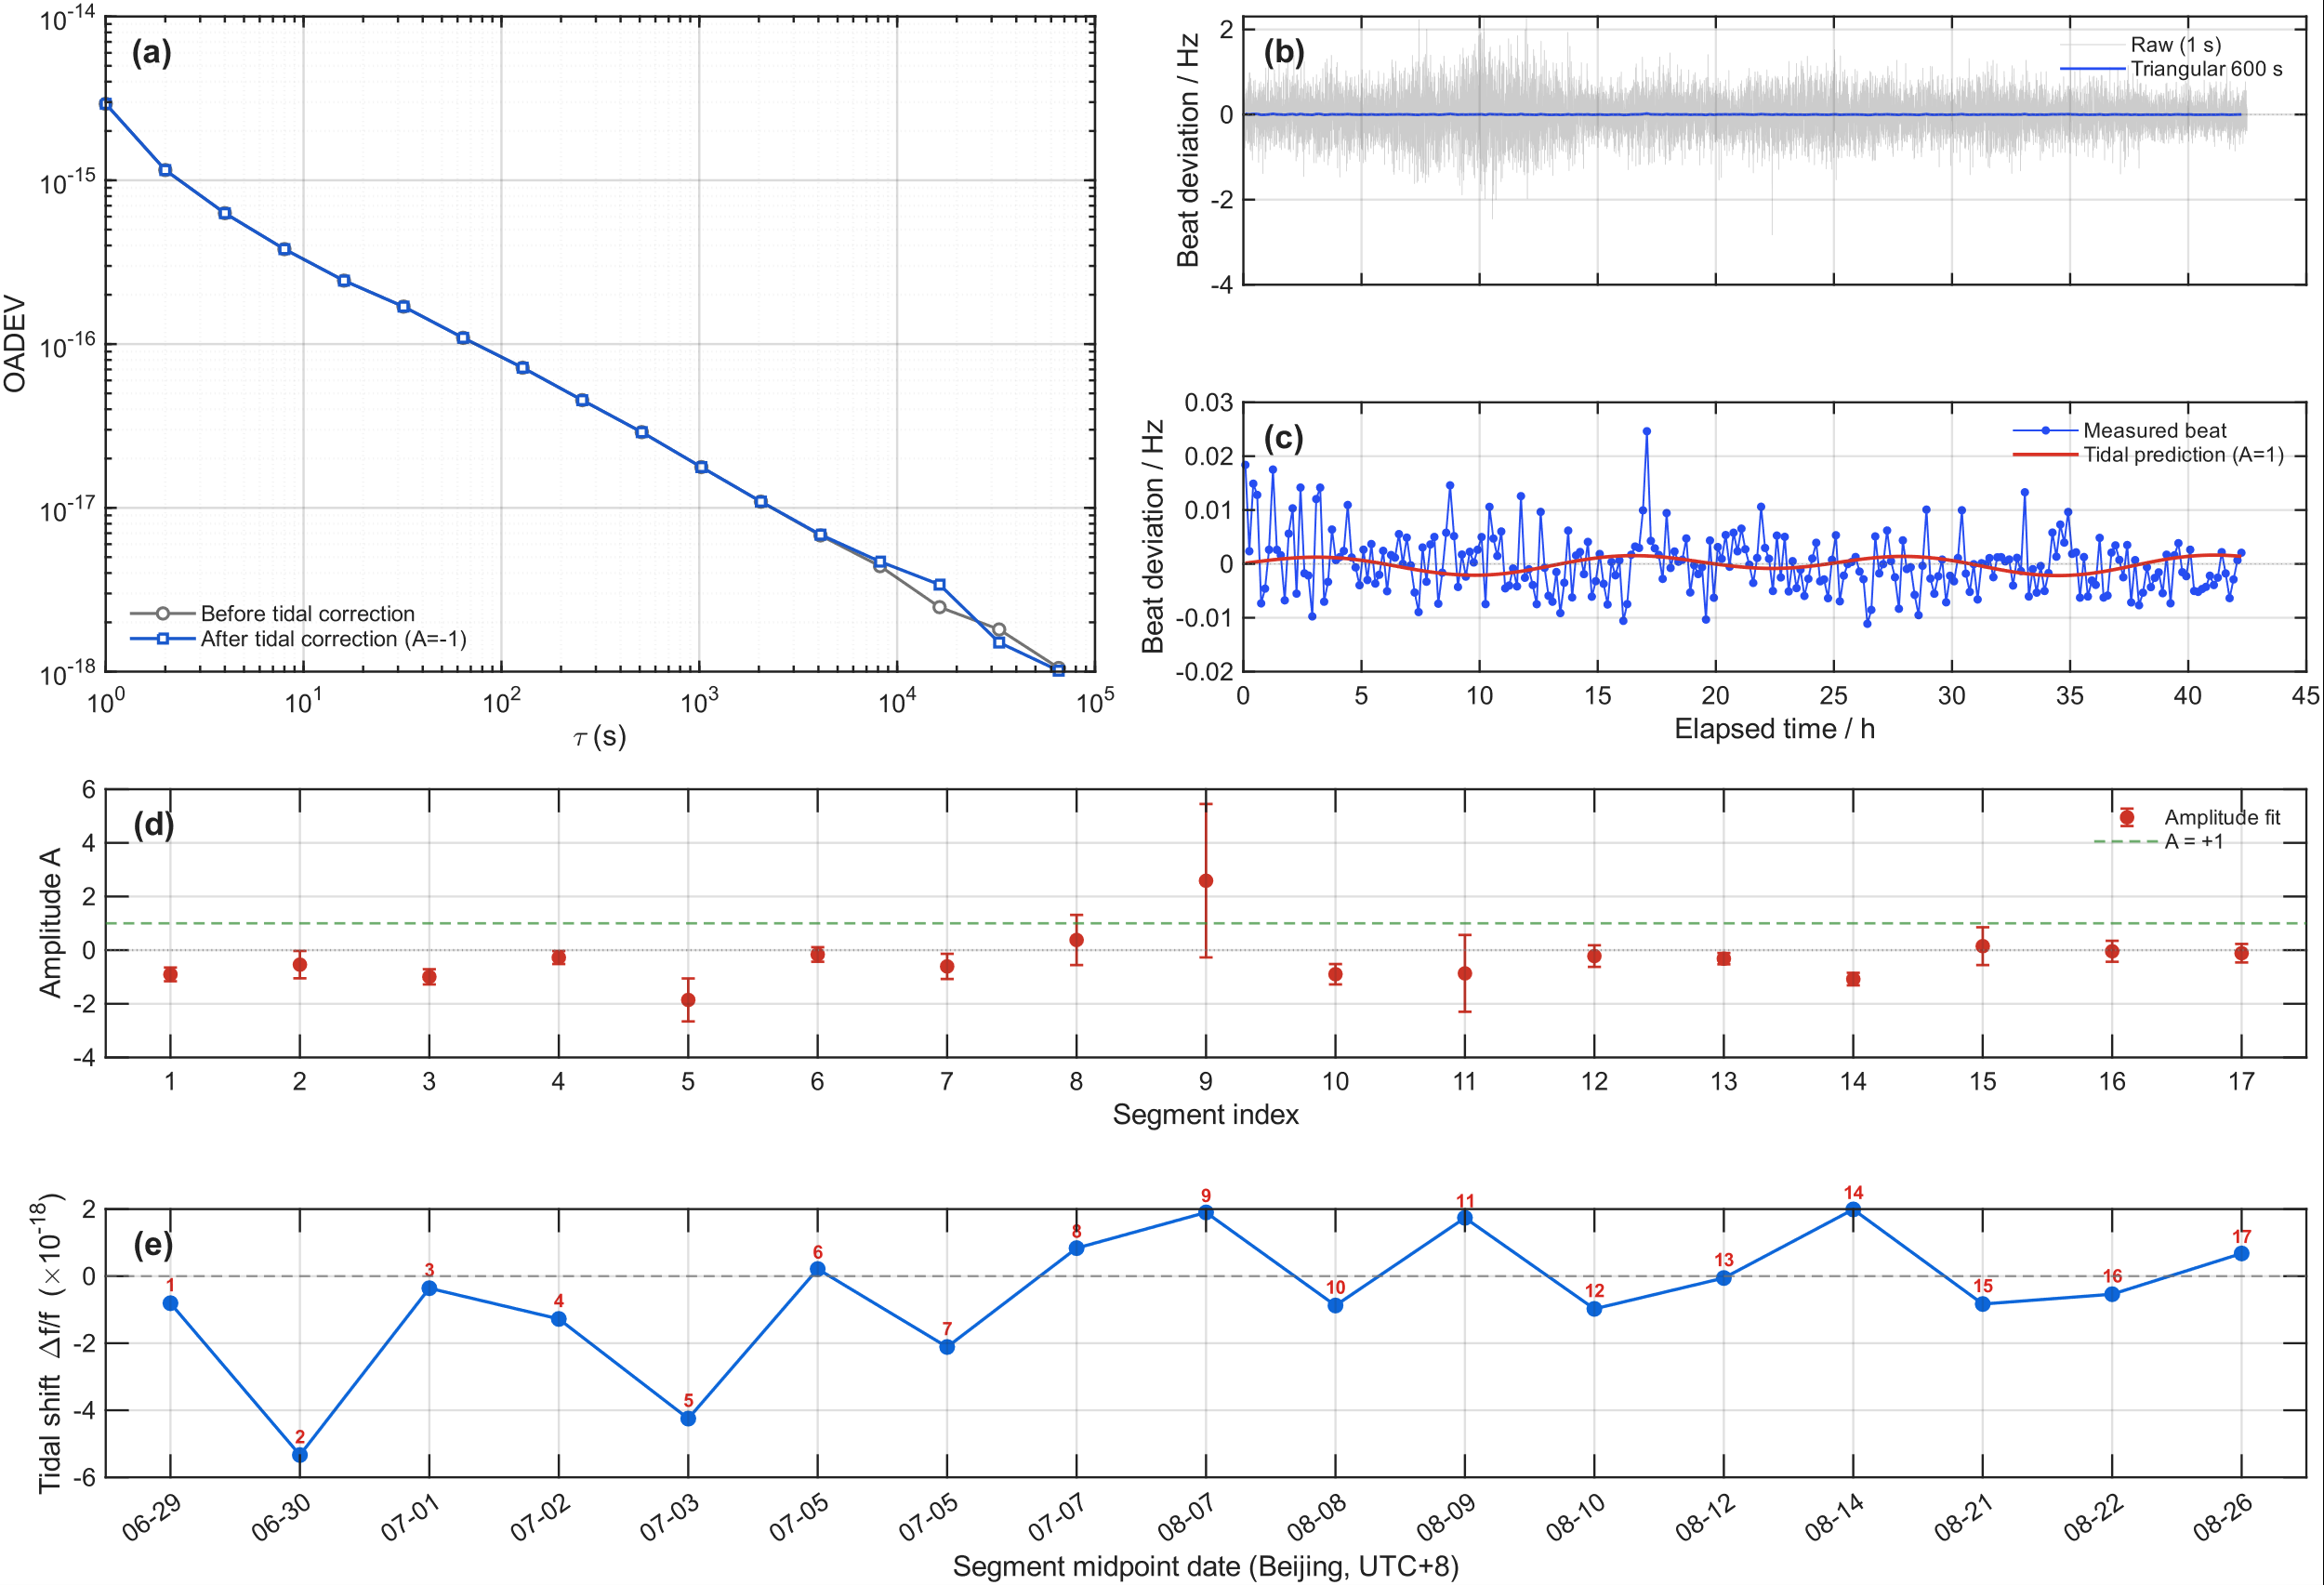
\includegraphics[width=0.95\linewidth]{figs/3.png}
  \caption{Tidal influence and its correlation. The 1200-s-window fit gives
    a historical amplitude estimate near $A=-0.54$ (about half the theoretical
    magnitude); overlapping-window significance is not interpreted as a
    detection statistic. At the segment-mean level the ratio
  deviation $y_i$ is positively correlated with the tidal shift
  $\dff$ (Pearson $r=+0.429$).}
  \label{fig:tidal}
\end{figure}

% =====================================================================


% ===== Tidal effect and its compensation =====

\subsection{Tidal effect and its compensation}
\label{sec:tidal-theory}

At the full theoretical response ($A=-1$, complete trust in the tidal
data and in general relativity) the tide would shift the ratio by
$0.44\e{-18}$: in fractional-frequency terms the duration-weighted centre
would move from $1.207\,507\,039\,343\,337\,720\,369\,6$ (raw) to
$1.207\,507\,039\,343\,337\,720\,810\,8$. That is small against the
$0.88\e{-18}$ statistical term but comparable to the leading systematics,
so we do not correct the central value; the tidal term enters the budget
as an uncertainty item of $<5\e{-19}$, its size set by that full-response
shift (Table~\ref{tab:budget}).
% src: clock_ratio/tidal_correction/summary.json
%      (R_duration raw 1.2075070393433377203696, theory 1.2075070393433377208108;
%       delta_R theory = 4.411914456944042e-19)

We asked whether an empirical response below the theoretical $A=-1$ is
justified. The measured amplitude is $A=-0.54\pm0.08$
(Sec.~\ref{sec:detection}), roughly half the theoretical magnitude, but
no independent check establishes the fitted value as the correct response
coefficient: the fit reproduces the waveform, not the hardware phase that
fixes the sign convention. We therefore do not adopt it as a compensation.

A half-strength response admits several physical readings, none of which
the present data can single out. The professional tidal series combines
solid-Earth tide with ocean loading, yet the loading term over a
\qty{700}{km} inter-city baseline depends on the local coastline and
sedimentary structure and on groundwater and hydrological loading that a
global model resolves only coarsely; a phase- or amplitude-mismatched
loading component would reduce the coherent response without removing it.
Alternatively, the two clocks sense slightly different local geopotentials,
and any common-mode environmental coupling along the fibre path that
partially tracks the tide would also dilute the fitted amplitude. Because
these mechanisms are degenerate at the present sensitivity, we keep the
uncorrected centre as the headline ratio and report the amplitude as an
effect estimate rather than a calibration, leaving a per-component tidal
model as the natural route to a full-strength response.

Compensating at the fitted $A=-0.54$ would shift the duration-weighted
centre by $+0.24\e{-18}$, half the $+0.44\e{-18}$ of the full theoretical
response, both below the present statistical uncertainty. Descriptively,
the empirical compensation would lower the reduced chi-square from
$3.91$ (raw) to $4.26$ and the segment-to-segment dispersion
$\sigma(y_i)$ from $2.580\e{-18}$ to $2.334\e{-18}$
($9.6\%$), while the full theoretical response gives a larger
$\sigma(y_i)$ reduction to $2.473\e{-18}$ ($4.2\%$) but a slightly
\emph{higher} $\chi^{2}_{\mathrm{red}}$ ($3.91\to4.11$); neither removes the
residual at long averaging times. These are
descriptive changes in scatter, not a validated correction: because
neither the statistics nor the sign convention establishes it, the
amplitude is reported as an effect estimate rather than adopted
(Supplementary Information).
% seg9: 16-segment values from clock_ratio/statistical_methods_tidal_seg9_excluded.json
%      (raw chi2_red 3.913 -> theory 4.113 / empirical 4.257;
%       sigma(y_i): raw 2.5805 -> theory 2.4730 / empirical 2.3336)

% =====================================================================


% =====================================================================
\section{Discussion}
\label{sec:caveats}

Two features set this network apart. It is inter-city and cross-species:
two clock species \citep{zhu2026yb, jia2026sr}, at two institutions and
two cities, joined only by the fibre link and the combs, yet yielding a
ratio that agrees with the leading independent determinations at the
$5\e{-18}$ level without any transport of the clocks. And the same data
set provides a time-varying-potential template response for further
covariance-aware study; the $0.88\e{-18}$ statistical floor corresponds to
an equivalent height of about $0.8$\,cm.

The comparison places the Yb/Sr ratio on the map of independent
determinations (Table~\ref{tab:compare}, Fig.~\ref{fig:compare}). Our
uncorrected centre lies
$-2.9\e{-18}$ below the NIST--JILA value \citep{aeppli2026nist} and
$+2.1\e{-18}$ above the European-network value
\citep{pizzocaro2026european}. The NIST--JILA determination carries a total
uncertainty at the few-parts-in-$10^{18}$ level, so our difference from it
is below the $5\e{-18}$ target; the European-network central value is
quoted for completeness rather than as an independent agreement test,
since its statistical uncertainty is substantially larger, and the
near-coincidence of the three values should not be read as a three-way
agreement at $5\e{-18}$. The choice of uncorrected or tidal-corrected
centre and of Bayesian or duration-weighted averaging moves any of these
deviations by at most $\sim0.7\e{-18}$, below the scale of interest.

The immediate metrological value of this work is as an independent check
on the Yb/Sr ratio that the redefinition of the SI second will rest on.
That redefinition calls for a matrix of ratios measured by different
laboratories and mutually agreeing at the few-parts-in-$10^{18}$ level;
for Yb/Sr only a single determination to date meets the $5\e{-18}$ target
\citep{aeppli2026nist}, and it differs markedly from earlier reports. The
present result adds a second, independently obtained entry to that
matrix, from a third institution with a different pair of clocks and
separate hardware and analysis, and so tests the redefinition on evidence
the single-campus determination cannot provide. We stress that this is a
conservative claim: the $0.88\e{-18}$ figure is a statistical floor, and
we report a ratio consistent with the existing determinations rather than
a new most-precise value.

The same data set also bounds what the comparison can support. The
bottleneck is no longer the link or the comb, whose contributions are each
below $1\e{-19}$ (Table~\ref{tab:budget}), but the segment-to-segment
scatter; closing the gap between the $0.88\e{-18}$ statistical floor and
the $\sim5\e{-18}$ spread between independent determinations therefore
requires progress on the systematic side, in the clock evaluations
\citep{zhu2026yb, jia2026sr} and in joint geodetic levelling, rather than
longer integration alone. Two further limits should be read with the
result: the per-segment uncertainties $u_i$ are unreliable (an OADEV
extrapolation that underestimates by roughly $30$--$40\%$, with anomalous
segments 5, 6 and 16), so the combined values are for method comparison
only; and the negative sign of the fitted amplitude is a specified
response convention rather than a resolution of the hardware-polarity
question.
% src: docs/METHODOLOGY.md Sec. 2.2, 9.5-9.6; clock_ratio/statistical_methods_tidal.json

\begin{table}[t]
  \centering
  \caption{Yb/Sr frequency-ratio determinations. Deviations are given
  relative to the present work (uncorrected centre, Sec.~\ref{sec:methods}),
  in units of $10^{-18}$.}
  \label{tab:compare}
  \begin{tabular}{lccc}
    \toprule
    Determination & Yb/Sr & Deviation & Ref. \\
    \midrule
    NIST--JILA       & $1.207\,507\,039\,343\,337\,7230(37)$ & $-2.9$ & \citep{aeppli2026nist} \\
    This work        & $1.207\,507\,039\,343\,337\,720\,1(29)$ & $0$    & --- \\
    European network & $1.207\,507\,039\,343\,337\,718(32)$  & $+2.1$ & \citep{pizzocaro2026european} \\
    \bottomrule
  \end{tabular}
  % seg9: 16-segment "this work" ratio ...7201(29); deviations vs NIST/EUR recomputed
  %      in Decimal80: 1.2075070393433377201 - 1.2075070393433377230 = -2.90e-18,
  %                     1.2075070393433377201 - 1.207507039343337718  = +2.10e-18.
\end{table}

\begin{figure}[t]
  \centering
  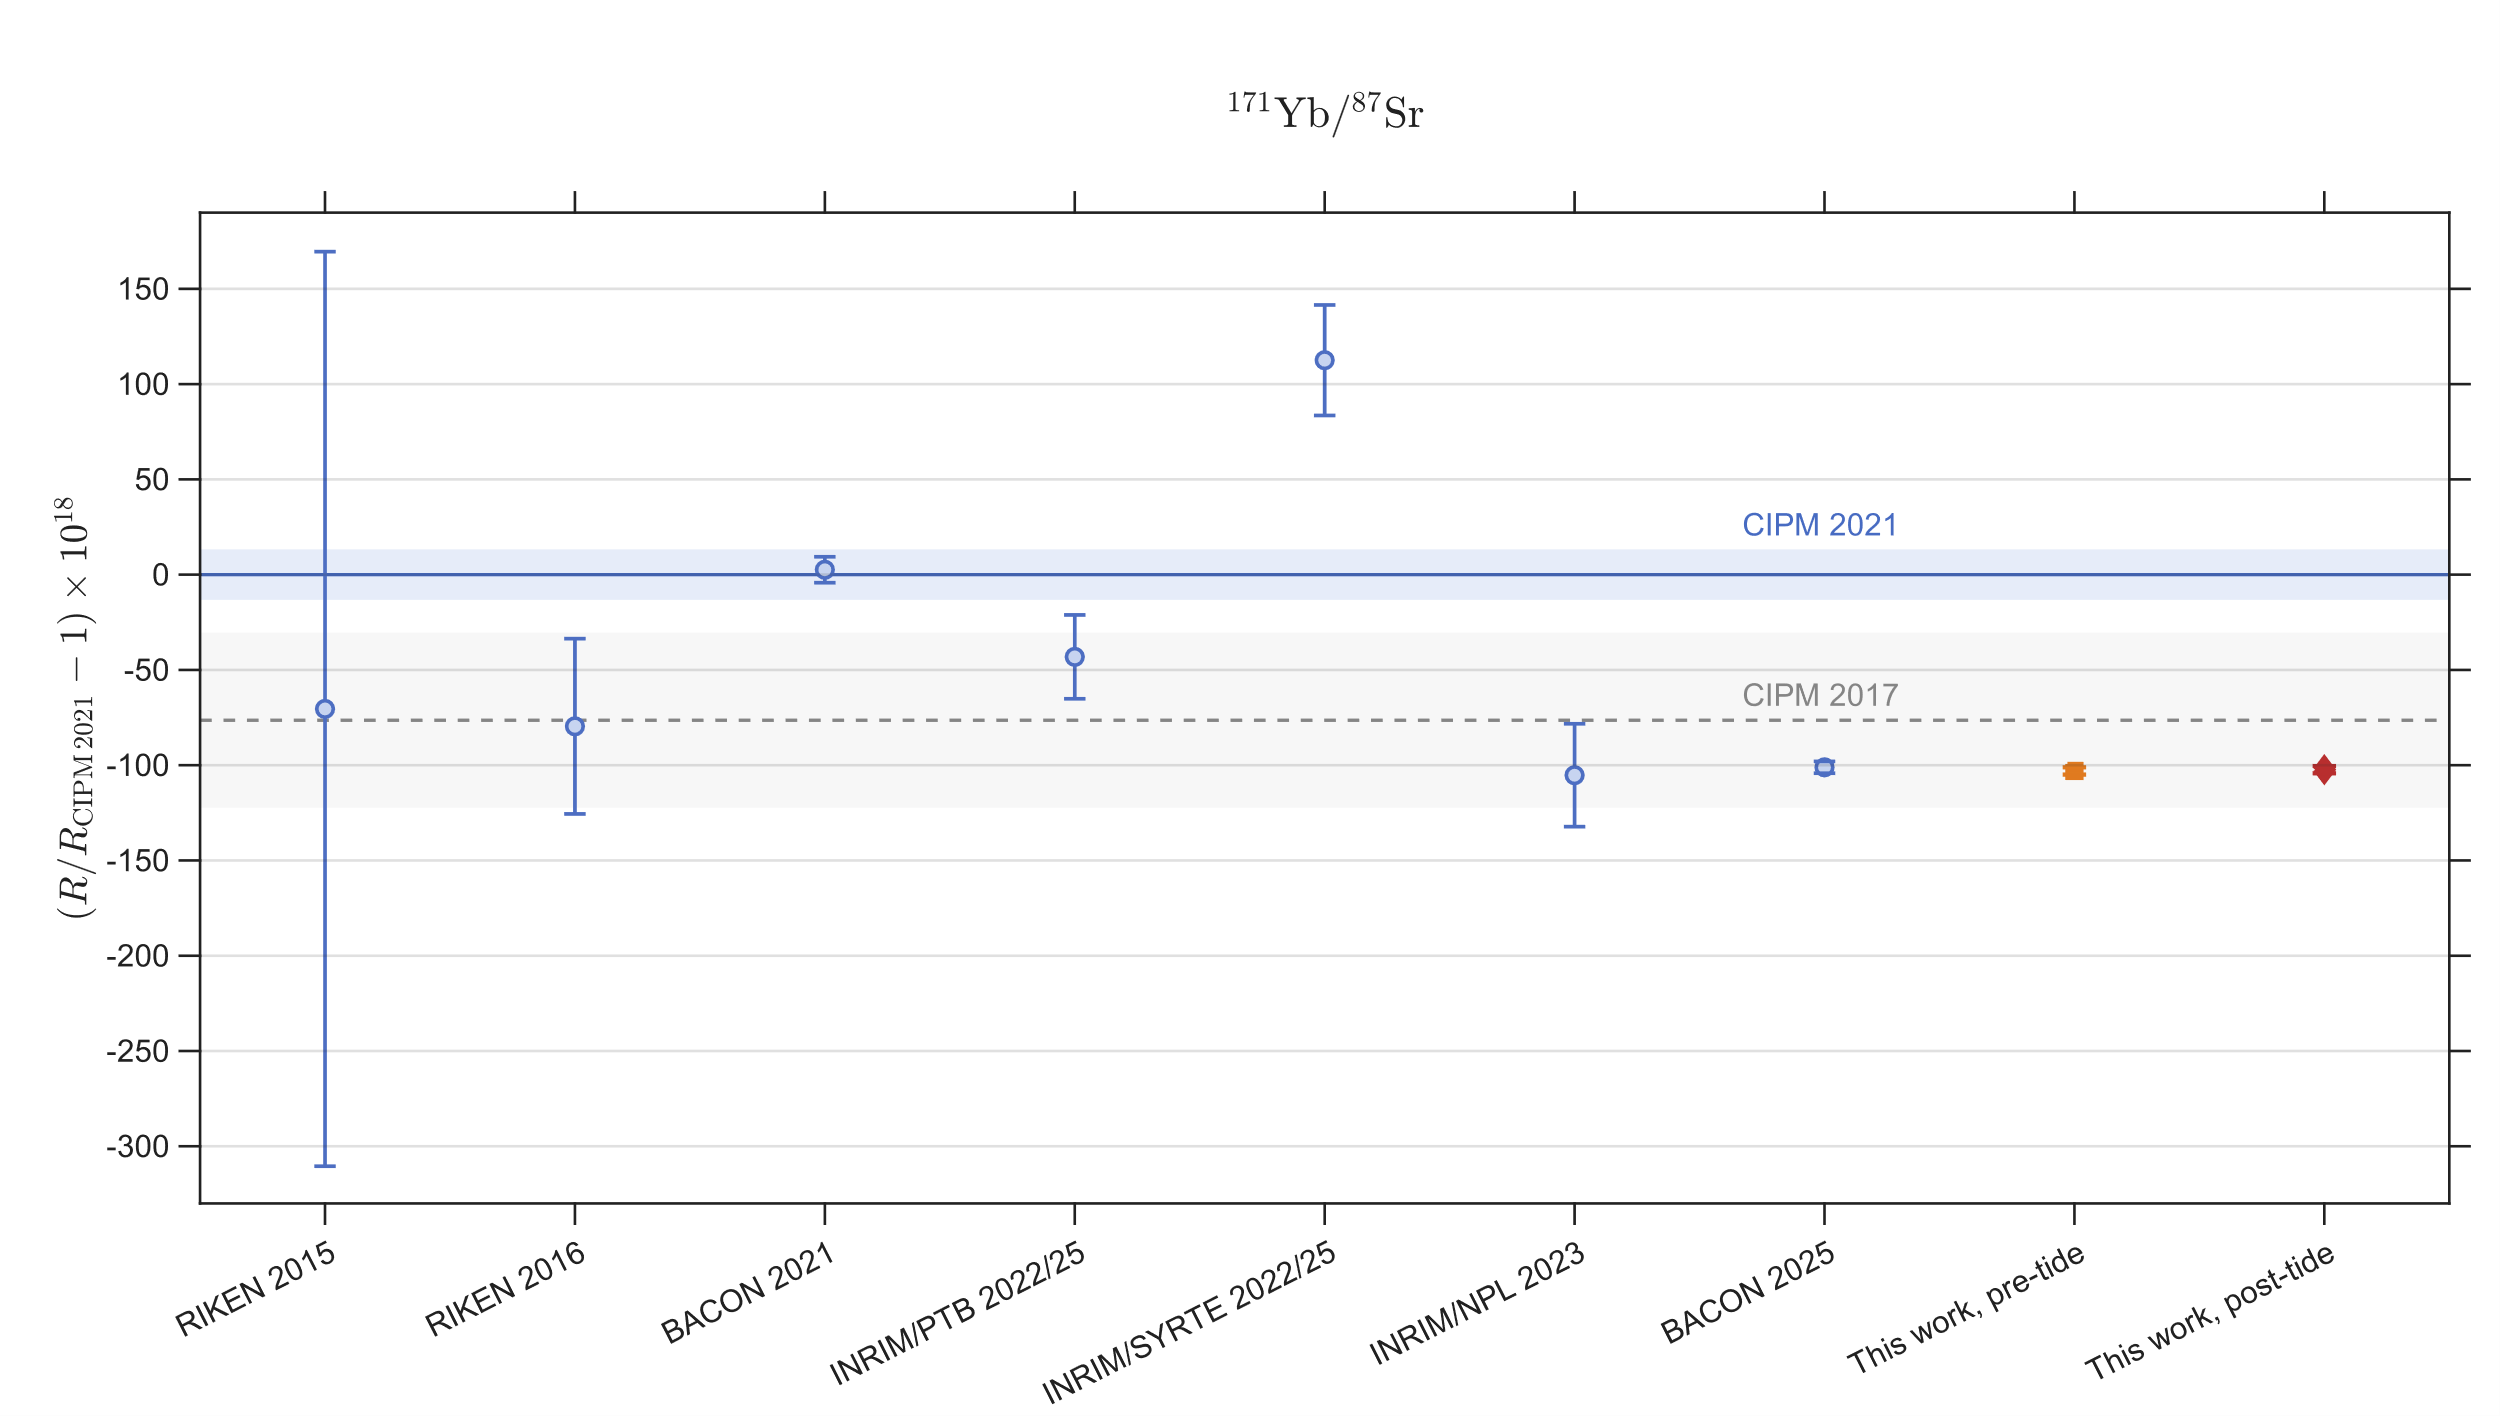
\includegraphics[width=0.95\linewidth]{figs/4.png}
  \caption{Comparison with previous determinations of the Yb/Sr ratio.
  The combined centres of this work, with the experiment-side WLS and
  NIST reference values, place the present result alongside the existing
  independent determinations.}
  \label{fig:compare}
\end{figure}

% =====================================================================
\section{Outlook}
\label{sec:outlook}

Beyond metrology, the same comparison is a candidate sensor for
chronometric geodesy: the ratio and the geopotential difference are read
from one measurement, and the tidal analysis here demonstrates the
required sensitivity on a single baseline. A genuine relativistic
coordinate reference frame, however, would require several nodes with
closing loops, geodetic ties, a frame convention and continuous
operation; a two-node, single-baseline, $\sim20\%$ duty-cycle experiment
is the elementary link of such a network, not the network itself.
Extending this prototype node pair to a multi-node network, with improved
link and comb stability and dedicated joint levelling, is the natural
next step.

Beyond geodesy, the same network reaches into fundamental physics, where
clock comparisons constrain dark-matter couplings \citep{wcislo2018global,
roberts2017domain} and test Lorentz symmetry \citep{sanner2019lorentz};
realizing that reach on an inter-city baseline is an open question
motivated by the present sensitivity.
% Position per paper/physics_analysis/NATURE_FRAMEWORK.md Sec. 1.

% =====================================================================
\section{Conclusion}
\label{sec:conclusion}

We have demonstrated an inter-city, cross-species optical-clock network:
an IAPMST Yb clock in Wuhan \citep{zhu2026yb} and a USTC Sr clock in
Shanghai \citep{jia2026sr}, about \qty{700}{km} apart and linked by a
phase-stabilised fibre, operated coherently for $58$\,days. Combining
$16$ segments with a Bayesian random-effect model gives an uncorrected
Yb/Sr ratio of $1.207\,507\,039\,343\,337\,720\,1(29)$ with a total
uncertainty of $2\e{-18}$, consistent with the existing determinations at
the $5\e{-18}$ level. The tidal gravitational-redshift template response is
carried as an uncertainty item, pending a covariance-aware detection analysis.
Two capabilities follow. The comparison supplies an independently
obtained entry for the Yb/Sr ratio that a redefined SI second will rest
on. And, for the first time over a real \qty{700}{km} baseline rather than a
single campus, the two independent clocks resolve the time-varying
gravitational potential at a centimetre-level equivalent height, casting
the inter-city clock network as a prototype relativistic-geodesy sensor
as well as a metrological one.

% =====================================================================
\section{Methods}
% =====================================================================

We describe the measurement and its analysis in three groups: the
apparatus and the link (§``Experimental setup and frequency transfer''),
the data set (§``Observation campaign and per-segment data''), and the
analysis chain that turns the raw beat into the reported ratio---the
ratio inversion, the systematic and geopotential corrections, the tidal
treatment, and the statistical combination of the per-segment results.

\subsection{Experimental setup and frequency transfer}
% =====================================================================

The main text keeps only the conceptual frequency chain; here we record
the symbol conventions that make the inversion reproducible. The
observable is the beat between the received \qty{1550}{nm} transfer carrier
and the local Yb-referenced comb; every frequency in the chain is derived
from the comb repetition rate $f_{\mathrm{rep}} =
f_{\mathrm{ref}}\times\mathrm{DIV20} = 200$\,MHz.
% src: clock/params.json (FREF=1e7, DIV20=20); docs/METHODOLOGY.md Sec. 7

The fibre link itself is built on the cascaded,
bias-corrected optical-frequency-dissemination architecture of
Ref.~\citep{chen2026dissemination}: the route is divided into segments,
each terminated by a relay station that carries a bidirectional
erbium-doped fibre amplifier and a fibre-noise-cancellation loop, with the
round-trip phase noise measured in the radio-frequency domain. Deployed
on paired strands within a single telecommunications cable duct, the
present Shanghai--Wuhan route is shorter than the \qty{2067}{km} field link of
Ref.~\citep{chen2026dissemination}, so the accumulated link noise is
correspondingly lower; the relay stations used here operate without the
dedicated sub-hertz noise-purification stage that the longer link
requires.

At the Shanghai end the Sr clock at \qty{698}{nm} is transferred to a
\qty{1397}{nm} carrier; at the Wuhan end a second comb links the received
\qty{1550}{nm} carrier to the Yb clock at \qty{578}{nm} through a \qty{1156}{nm}
fundamental beam. The clock-laser frequency relations are
\begin{align}
  f_{\mathrm{comb}}^{1397} &= \tfrac{1}{2}\,(1+a)\,f_{\mathrm{Sr}},
  \qquad a = a_{\mathrm{dens}} + a_{\mathrm{lat}} + a_{Z^2} + a_{\mathrm{BGC}}, \\
  f_{\mathrm{comb}}^{1156} &= \tfrac{1}{2}\,(1+b)\,f_{\mathrm{Yb}},
\end{align}
where $a$ collects the Sr-side systematic corrections \citep{jia2026sr} and
$b$ the Yb-side correction \citep{zhu2026yb} ($b_{\mathrm{Yb}} =
-1.7\e{-18}$; the internal components are listed below and in the
repository). Table~\ref{tab:aom} gives the AOM frequency offsets and
their roles in the link and comb chains.
% src: clock/params.json (B_YB); docs/METHODOLOGY.md Sec. 1.2;
% src: experiment-side manuscript (光钟比对论文 hj.docx, supplementary S1)

\begin{table}[t]
  \centering
  \caption{AOM frequency offsets and their roles in the
  Shanghai--Wuhan link and comb chains (from the experiment-side
  supplementary material). FNC denotes a fibre-noise-cancellation loop;
  BBR a blackbody-radiation correction loop.}
  \label{tab:aom}
  \begin{tabular}{cl}
    \toprule
    Index & Offset and role \\
    \midrule
    1  & $+80$\,MHz, fixed \\
    2  & $+80.274$\,MHz, FNC $+$ closed-loop feedback \\
    3  & $+80$\,MHz, FNC $+$ BBR feedback \\
    4  & $-110$\,MHz, FNC feedback \\
    5  & $+50$\,MHz, FNC feedback \\
    6  & $+236$\,MHz, clock-laser--cavity offset; cavity feed-forward \\
    7  & $-80$\,MHz, FNC feedback \\
    8  & $+155$\,MHz, frequency compensation and correction \\
    9  & $-80$\,MHz, FNC feedback \\
    10 & $+105$\,MHz, frequency compensation and correction \\
    11 & $+80$\,MHz, FNC feedback \\
    12 & $-140$\,MHz, clock interrogation control \\
    a  & $+50$\,MHz, feedback, fibre transfer FNC \\
    b  & $-40$\,MHz, fixed \\
    \bottomrule
  \end{tabular}
\end{table}

The static geopotential difference between the two clocks,
$\dW = 280.04164\ \mathrm{m^{2}/s^{2}}$, is applied at the ratio level as a
constant correction $\delta_g = \dW/c^{2} = -3.1159\e{-15}$ (fixed by the
levelling described below):
$\mathrm{(Yb/Sr)}_{\mathrm{corr}} = \mathrm{(Yb/Sr)}_{\mathrm{raw}}
\times (1+\delta_g)$.
% src: paper/武汉-上海水准测量0930R1.docx (Delta_W = 280.04164 m^2/s^2);
%      delta_g = Delta_W/c^2

% =====================================================================


\subsection{Observation campaign and per-segment data}
\label{app:segments}
% =====================================================================

The comparison spans the $58$-day campaign described in the main text.
Table~\ref{tab:segments} lists the 16 uninterrupted segments used in this
variant (segment~9 excluded), their
retained sample counts $n_i$ (after endpoint trimming) and measurement
campaign; the retained total is $\sum_i n_i = 986\,416$ one-second
samples. During campaign~1 the Yb and Sr clocks were restarted
independently between some segments (Yb after segments 4--6; Sr after
segments 7--8), which lets the reproducibility of the ratio be checked
directly.
% seg9: segment 9 removed; retained total 986 416 s = 1 008 912 - 22 496
% src: clock_ratio/ratio_17seg.csv (n_valid); clock_ratio/statistical_methods_tidal_seg9_excluded.json

\begin{table}[t]
  \centering
  \caption{The 16 uninterrupted segments (segment 9 excluded): index,
  retained samples $n_i$ (endpoint-trimmed), and Beijing-time start.}
  \label{tab:segments}
  \begin{tabular}{ccl}
    \toprule
    Segment & $n_i$ (s) & Start (Beijing) \\
    \midrule
    1  & $68\,009$  & 2026-06-29 10:06:28 \\
    2  & $29\,481$  & 2026-06-30 12:00:01 \\
    3  & $42\,891$  & 2026-07-01 15:58:41 \\
    4  & $64\,280$  & 2026-07-02 14:00:01 \\
    5  & $19\,532$  & 2026-07-03 17:34:22 \\
    6  & $52\,140$  & 2026-07-04 19:30:46 \\
    7  & $39\,526$  & 2026-07-05 13:00:01 \\
    8  & $43\,565$  & 2026-07-06 21:45:16 \\
    10 & $57\,938$  & 2026-08-07 22:15:00 \\
    11 & $35\,824$  & 2026-08-09 00:00:00 \\
    12 & $40\,346$  & 2026-08-10 12:47:06 \\
    13 & $152\,994$ & 2026-08-11 05:30:00 \\
    14 & $68\,618$  & 2026-08-13 18:56:58 \\
    15 & $57\,649$  & 2026-08-21 00:40:03 \\
    16 & $147\,640$ & 2026-08-21 23:20:01 \\
    17 & $65\,983$  & 2026-08-25 15:09:41 \\
    \midrule
    \multicolumn{1}{r}{Total} & $986\,416$ & \\
    \bottomrule
  \end{tabular}
  % seg9: row 9 (22 496 s) removed from the 17-segment table.
  % src: clock_ratio/ratio_17seg.csv; segment windows in clock/params.json.
\end{table}

% =====================================================================


\subsection{Beat-to-ratio inversion}
\label{app:methods-ratio}
We take $b_i(t)$ as the longest valid beat sequence in segment $i$ and
$m$ as the global median of the plausible beat values, so the segment beat
deviation is
\begin{equation}
  \overline{\delta b}_i = \overline{b_i} - m .
\end{equation}
The Sr-side systematic shift $a_i$ and the Yb-side shift $b_{\mathrm{Yb}}$
combine into the Dr coefficient, and the segment Yb/Sr ratio follows from
the full inversion
\begin{equation}
  R_i = \bigl[\,\mathrm{ratio\_base}_i + \mathrm{Dr}_i\,\bigr]^{-1}
        \times (1+\delta_g),
  \qquad \delta_g = -3.1159\e{-15},
  \label{eq:ratio}
\end{equation}
where $\delta_g$ is the static gravitational correction. All ratio
arithmetic is carried out at 80-decimal precision (\texttt{Decimal80},
mirroring MATLAB \texttt{vpa(...,80)}); a float64 absolute precision of
about $2.6\e{-16}$ would destroy differences at the $10^{-18}$ level. The
duration-weighted centre of the whole experiment is
\begin{equation}
  \Rdur = \frac{\sum_i n_i R_i}{\sum_i n_i},
  \qquad \sum_i n_i = \num{986416}.
  \label{eq:rduration}
\end{equation}
% seg9: retained total 986 416 = 1 008 912 - 22 496 (segment 9 removed)
% src: docs/METHODOLOGY.md Sec. 1.3, docs/NOTATION.md Sec. 5;
%      delta_g = Delta_W/c^2 with Delta_W = 280.04164 m^2/s^2 (levelling doc)


\subsection{Systematic frequency shifts}
\label{app:systematics}

The ratio inversion removes the known systematic shifts of both clocks
through the coefficients $a_i$ (Sr side) and $b$ (Yb side). The Yb-side
correction is a fixed value, $b_{\mathrm{Yb}} = (5.3 - 7.0)\times10^{-18}
= -1.7\e{-18}$, entering as $\mathrm{coef}_{1156} = (1+b_{\mathrm{Yb}})/2$.
The Sr-side correction is segment-dependent and is the sum of five terms,
\begin{equation}
  a_i = a_{\mathrm{rou},i} + a_{\mathrm{AC},i} + a_{\mathrm{SM},i}
        + a_{\mathrm{air},i} + a_{\mathrm{BBR},i},
  \qquad \mathrm{coef}_{1397,i} = \tfrac{1}{2}(1+a_i),
  \label{eq:shifta}
\end{equation}
where $a_{\mathrm{rou}}$ is the lattice light-shift, $a_{\mathrm{AC}}$
the ac-Stark shift ($+7.444\e{-18}$ in the first campaign, $+8.929\e{-18}$
in the second), $a_{\mathrm{SM}}$ the second-order Zeeman shift
($\approx-1.78\e{-16}$ in the first campaign; $-8.925\e{-17}$ in segment 9
and zero in segments 10--14), $a_{\mathrm{air}}$ the air-refractivity
correction ($-6.7\e{-19}$) and $a_{\mathrm{BBR}}$ the blackbody-radiation
shift (zero). Segments 15--17 reuse the constant $a_i$ of segments
12--14. The per-segment values are stored in the repository
(\texttt{clock/params.json}); the anomalous \texttt{a\_SM} of segment~9 is
retained as delivered, without adjustment. The component evaluations
follow the published assessments of the two clocks
\citep{zhu2026yb, jia2026sr}.
% src: docs/NOTATION.md Sec. 5.1, clock/params.json (shift_a)


\subsection{Levelling determination of the geopotential difference}
\label{app:levelling}

The static gravitational-redshift correction $\delta_g$ entering the ratio
inversion is fixed by the geopotential difference between the two clocks'
atomic transition positions, determined by first-order spirit levelling
together with simultaneous gravimetry. A levelling line of about \qty{1113}{km}
was run between the Wuhan benchmark WS-03 (at IAPMST) and the Shanghai
benchmark WS-01 (at USTC), comprising six first-order routes through
Ezhou, Huangshi, Huanggang, Lu'an, Hefei, Wuhu, Guangde and Suzhou.
Levelling was performed with digital levels (Sokkia SDL1X, Trimble
DiNi03) and bar-coded invar staffs, with sight lengths below \qty{30}{m} and a
forward--back sight-length difference below \qty{1.0}{m}; gravity was
observed at every levelling point with two relative gravimeters. The
levelled normal heights were converted to orthometric heights for the
geopotential integration, and the geopotential difference between the two
benchmarks follows from $\dW_{AB} = -\sum_i g_i\,\Delta H_i$, where $g_i$
is the mean gravity and $\Delta H_i$ the orthometric height difference of
the $i$-th segment.

Two further segments connect each benchmark to the corresponding atomic
transition position: the benchmark-to-optical-platform height difference
was obtained by trigonometrical heighting (total station), and the
platform-to-atom segment from the clock design parameters. The five
partial geopotential differences are listed in Table~\ref{tab:levelling}
and sum to $\dW = 280.04164\ \mathrm{m^{2}/s^{2}}$ between the two atomic
transition positions. The levelling precision, expressed as the
accidental mean error per kilometre, is \qty{0.255}{mm}, better than the
\qty{0.45}{mm} limit for first-order levelling. Propagating the levelling,
trigonometrical-heighting and platform-to-atom terms yields a total
height precision of $\pm0.0086$\,m, and hence a geopotential-difference
uncertainty of $\pm0.085\ \mathrm{m^{2}/s^{2}}$.
% src: paper/武汉-上海水准测量0930R1.docx (Secs. 1-3; Delta_W = 280.04164 m^2/s^2,
%      sigma(W) = 0.085 m^2/s^2)

\begin{table}[t]
  \centering
  \caption{Partial geopotential differences between the Yb (Wuhan) and
  Sr (Shanghai) clocks, in $\mathrm{m^{2}/s^{2}}$.}
  \label{tab:levelling}
  \begin{tabular}{lr}
    \toprule
    Segment & $\Delta W$ ($\mathrm{m^{2}/s^{2}}$) \\
    \midrule
    Yb atom $\to$ Yb optical platform        & $+2.65399$ \\
    Yb platform $\to$ benchmark WS-03        & $-14.51715$ \\
    Benchmark WS-03 $\to$ benchmark WS-01    & $+296.33022$ \\
    Benchmark WS-01 $\to$ Sr optical platform & $-1.47246$ \\
    Sr platform $\to$ Sr atom                & $-2.95296$ \\
    \midrule
    Yb atom $\to$ Sr atom (total)            & $+280.04164$ \\
    \bottomrule
  \end{tabular}
  % src: paper/武汉-上海水准测量0930R1.docx (Table 1)
\end{table}

% =====================================================================


\subsection{Tidal analysis}
\label{app:tidal}

The tidal beat template is formed from the professional \qty{30}{s}
geopotential-difference series, linearly interpolated to the retained
beat timestamps after shifting the Beijing-time beat windows to UTC. It
is normalised to the \qty{1550}{nm} transfer frequency,
$h(t) = F_{1550}\,\dW(t)/c^{2}$ with
$F_{1550} = N_{1550}^{\mathrm{WH}} f_{\mathrm{rep}} = \qty{193.3992}{THz}$,
\emph{not} to $1/\mathrm{COEF}$, which would be larger by the Yb/Sr
factor $\approx 1.2075$ and would bias $A$ low by that factor. Within
each segment the beat and the template are passed through a \qty{1200}{s}
triangular window (\qty{600}{s} step) and, after demeaning, fitted with
$\mathrm{beat} = A\,\mathrm{tide} + \mathrm{noise}$,
$A = \sum(\mathrm{tide}\cdot\mathrm{beat})/\sum\mathrm{tide}^{2}$. The
resulting segment-mean correlation between $y_i$ and $\dff$ is shown in
Fig.~\ref{fig:corr-scatter}. We
combine the per-segment amplitudes by precision weighting, together with
the sign-consistency (binomial), signed Stouffer and Fisher summaries.
The inferential inputs use non-overlapping windows; no sign-agnostic
Stouffer significance is assigned.
% src: docs/METHODOLOGY.md Sec. 5.1-5.3, Sec. 9

For the fixed-coefficient scenarios we apply the correction to the beat
before re-inverting the ratio, $b_{\mathrm{corr}}(t) =
b_{\mathrm{raw}}(t) - A\,h(t)$ with $A=-1$ (theory) or $A=-0.54$
(empirical); the ratio chain is then re-inverted and the four combination
methods re-applied. The direction self-check and the dispersion reduction
are reported in the Results. Because the two amplitudes are fixed rather
than fitted, and the sign follows a specified response convention (see
Discussion), we report these scenarios as effect estimates and keep the
uncorrected centre as the headline ratio.

\begin{figure}[t]
  \centering
  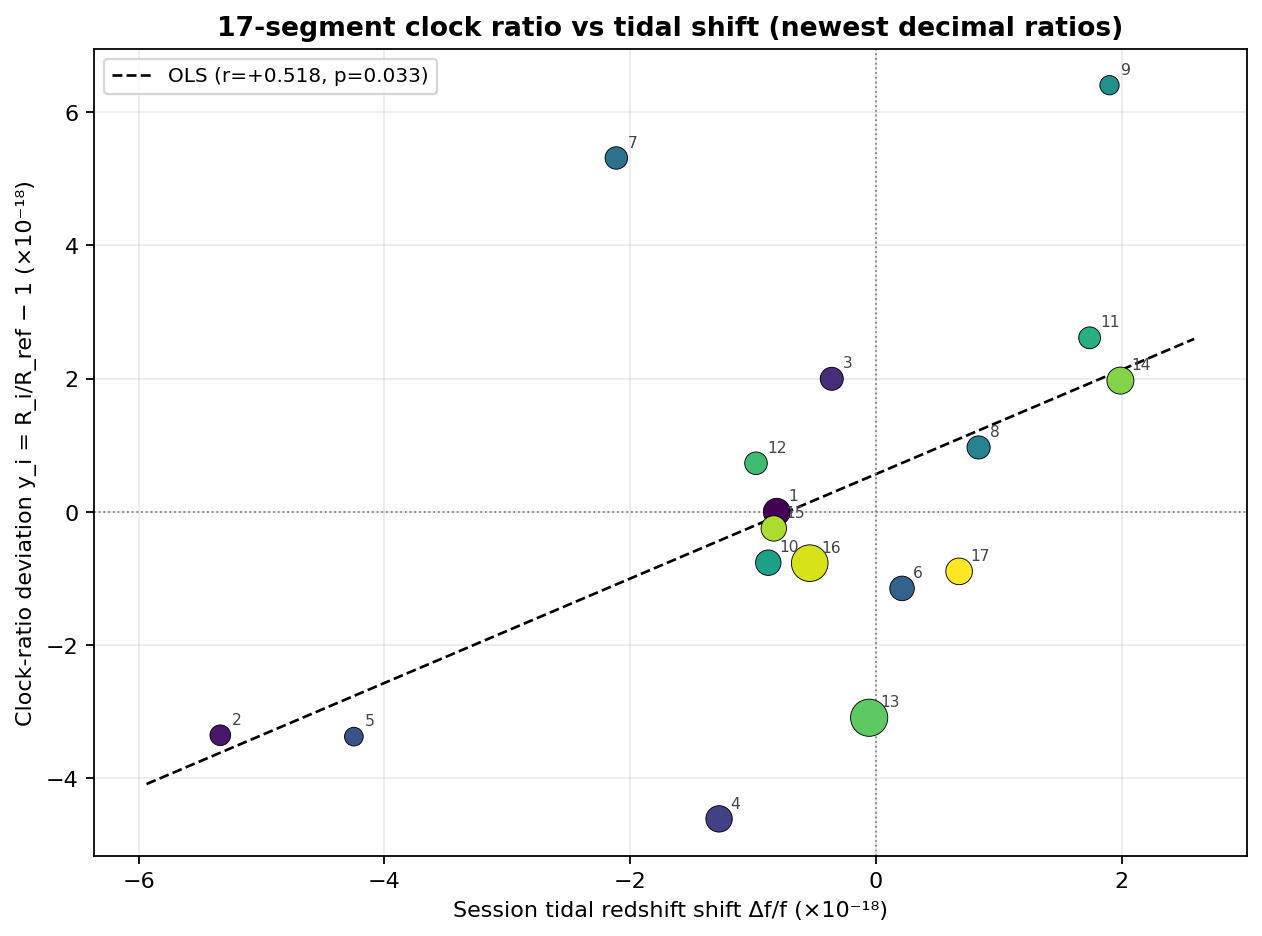
\includegraphics[width=0.75\linewidth]{figs/figS2_correlation.png}
  \caption{Segment-mean correlation. Clock-ratio deviation
  $y_i = R_i/R_{\mathrm{seg1}} - 1$ against the session tidal shift
  $\dff$ for the 16 segments (segment 9 excluded); the ordinary
  least-squares fit gives the positive correlation reported in the
  Results (Pearson $r=+0.43$, $p=0.098$).}
  \label{fig:corr-scatter}
\end{figure}


\subsection{Per-segment uncertainties}
\label{app:ui}

Each segment is assigned a statistical uncertainty from the overlapping
Allan deviation (OADEV) of its fractional frequency series
$\delta f/F_{1550}$. Over the white-frequency-noise range
$128\,\mathrm{s} \le \tau \le T/4$ the OADEV follows
$\sigma_y(\tau) \propto \tau^{-1/2}$; a linear fit of
$\log\sigma_y$ against $\log\tau$ is extrapolated to the segment length
$T$ to give $\sigma_y(T)$, and
\begin{equation}
  u_i = \sigma_y(T)\,R_i
  \label{eq:ui}
\end{equation}
is the absolute segment uncertainty on $R_i$.
% src: docs/METHODOLOGY.md Sec. 2.2-2.3
A flicker floor beyond $\tau \sim 4096$\,s makes this extrapolation
underestimate the $u_i$ (see Discussion). This is why we compare four
combination methods instead of adopting a single $u_i$-weighted mean, and
why the excess-scatter term $\xi$ below is required rather than optional.
The long-averaging-time behaviour is shown by the overlapping Allan
deviation of the seventeen segments spliced end-to-end on one continuous
\qty{1}{s} record (gaps removed), for the raw, theory and empirical
scenarios, with Riley--Howe effective-degrees-of-freedom error bars
(Fig.~\ref{fig:stability-long}).
% src: clock_ratio/concatenated_stability_long.{md,csv}

\begin{figure}[t]
  \centering
  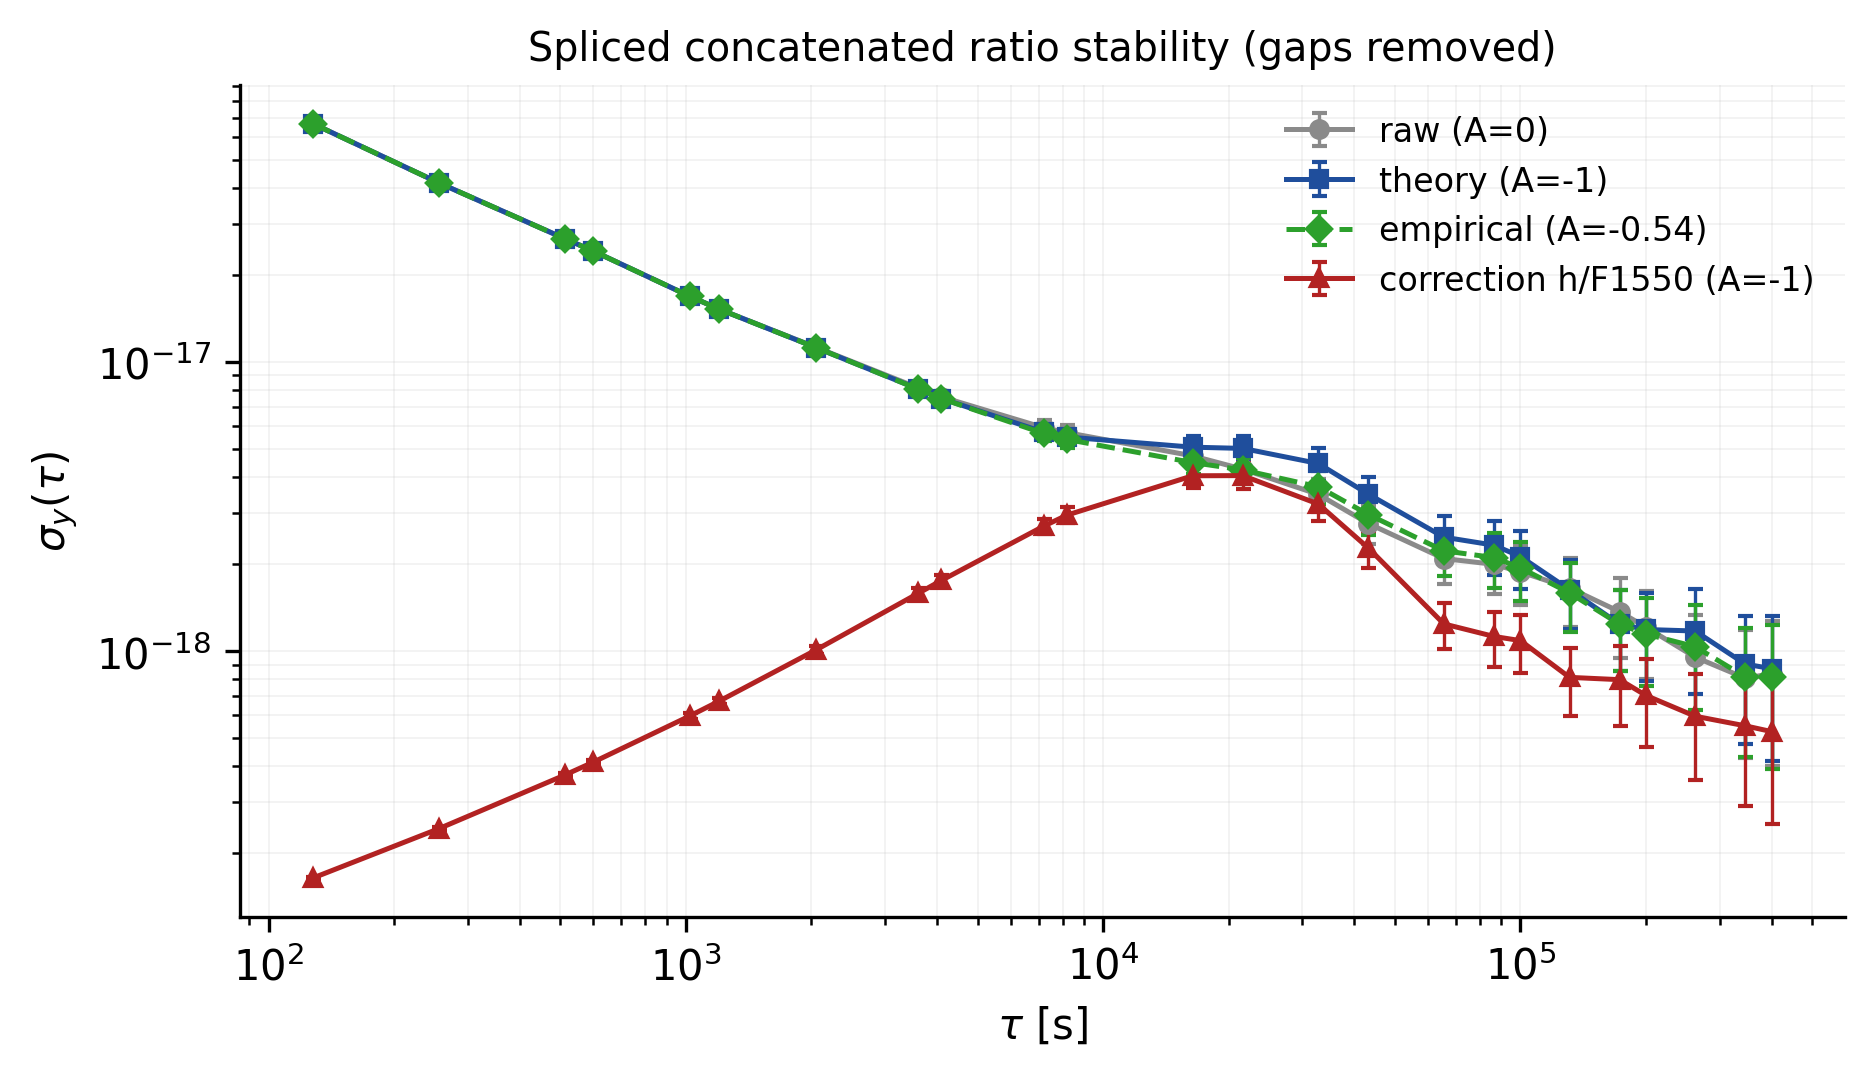
\includegraphics[width=0.85\linewidth]{figs/figS3_stability_long.png}
  \caption{Spliced concatenated stability. Overlapping Allan deviation
  $\sigma_y(\tau)$ of the seventeen segments placed end-to-end on one
  continuous \qty{1}{s} record (aligned pure-data span $11.7$\,d, gaps
  removed; $\tau$ up to $4.63$\,d), for the raw ($A=0$), theory
  ($A=-1$) and empirical ($A=-0.54$) scenarios, with the correction-term
  curve and Riley--Howe EDF error bars.}
  \label{fig:stability-long}
\end{figure}


\subsection{Statistical combination methods}
\label{app:methods}

The inter-segment scatter exceeds what the per-segment uncertainties
$u_i$ alone can explain, so the final ratio is obtained with a
random-effect model rather than a fixed-effect average. On the same
per-segment $(R_i, u_i)$ input we compare four combination methods, both
for the uncorrected baseline and for the two tidal-correction scenarios
(Sec.~\ref{app:tidal}):
\begin{itemize}
  \item \textbf{WLS (fixed effect)}: weights $w_i = 1/u_i^{2}$, no
        extra scatter; the $u_i$ are taken at face value.
  \item \textbf{Birge}: the $u_i$ are rescaled by a single factor
        $B = \sqrt{\chi^{2}_{\mathrm{red}}}$.
  \item \textbf{Mandel--Paule}: a common excess random variance
        $\xi^{2}$ is added, $\sigma_i^{2} = u_i^{2} + \xi^{2}$, with
        $\xi$ solved as a fixed value.
  \item \textbf{Bayesian hierarchical}: the same observation model as
        Mandel--Paule, but $\mu$ and $\xi$ are both inferred, so the
        uncertainty of $\xi$ propagates into the final ratio through the
        joint posterior (sampled by MCMC).
\end{itemize}
All four methods give consistent central values, and the statistical
uncertainty grows monotonically from WLS through Birge and Mandel--Paule
to Bayesian (Table~\ref{tab:appendix-methods}); we adopt the Bayesian
result as the primary statistical uncertainty. The direction of change
under the tidal correction is the same for all four methods.
% src: clock_ratio/statistical_methods_tidal.json (synthesis.methods)

\begin{table}[t]
  \centering
  \caption{Centre and statistical uncertainty by combination method for
  the uncorrected baseline, computed in this work's own re-run of the
  16-segment ratios (segment 9 excluded), in units of $10^{-18}$
  (deviations relative
  to the experiment-side WLS reference $1.207\,507\,039\,343\,337\,721\,3$).
  The experiment-side analysis reports a slightly different Bayesian
  statistical term ($0.88\times10^{-18}$; adopted for this variant's
  headline value), reflecting its own ratio pipeline.}
  \label{tab:appendix-methods}
  \begin{tabular}{lcc}
    \toprule
    Method & Centre deviation & Statistical $u$ \\
    \midrule
    WLS (fixed effect)       & $-1.152$ & $0.286$ \\
    Mandel--Paule            & $-0.661$ & $0.785$ \\
    Bayesian hierarchical    & $-0.656$ & $0.879$ \\
    \bottomrule
  \end{tabular}
  % seg9: 16-segment values from clock_ratio/statistical_methods_tidal_seg9_excluded.json
  %      (scenarios.raw: u_wls=2.858e-19, u_mp=7.852e-19, u_stat_bayes=8.791e-19)
\end{table}

% =====================================================================


\subsection{Statistical model details}
\label{app:stats}
% =====================================================================

Section~\ref{app:methods} introduced the four combination methods. Here
we record the shared observation model and the convergence diagnostics.
All four methods assume
\begin{equation}
  R_i \sim \mathcal{N}\!\left(\mu,\ u_i^{2} + \xi^{2}\right),
  \label{eq:obs}
\end{equation}
where $\mu$ is the common true ratio and $\xi$ the excess
segment-to-segment scatter not described by the per-segment OADEV
uncertainties $u_i$. The Bayesian hierarchical model treats both $\mu$
and $\xi$ as unknown and infers their joint posterior,
\begin{equation}
  p(\mu,\xi \mid D) \propto p(D \mid \mu,\xi)\,p(\mu)\,p(\xi),
  \qquad
  p(D\mid\mu,\xi) = \prod_i
    \frac{1}{\sqrt{2\pi(u_i^{2}+\xi^{2})}}\,
    e^{-\frac{(R_i-\mu)^{2}}{2(u_i^{2}+\xi^{2})}},
  \label{eq:bayes}
\end{equation}
with $D = \{R_i, u_i\}$. Because $\xi$ is a random parameter, its
posterior uncertainty propagates into the final ratio, unlike
Mandel--Paule, which first fixes a point estimate of $\xi$ and then
averages.
% src: docs/METHODOLOGY.md Sec. 3.3-3.4; clock_ratio/statistical_methods.py

The posterior is sampled by MCMC. Multiple independent chains mix over
the full sampling range with no long-term drift or inter-chain
separation, and the Gelman--Rubin convergence diagnostic,
$\hat{R}_{\mu} = \hat{R}_{\xi} = 1.000$, confirms convergence to a common
posterior. The final ratio is the posterior mean of $\mu$, with the
posterior standard deviation as the statistical uncertainty and the $68\%$
credible interval taken from the posterior.
% src: experiment-side manuscript (光钟比对论文 hj.docx, supplementary S3.4)

% =====================================================================


\section*{Funding}
% =====================================================================
% PLACEHOLDER: to be completed before submission. List the funding sources
% and grant numbers that directly supported this work. Declare funding here
% only when the work falls within the scope of, and arose directly from, the
% named grant.
% =====================================================================


\section*{Author contributions}
% =====================================================================
% PLACEHOLDER: to be completed by the collaboration before submission,
% following the CRediT taxonomy (conceptualization, methodology, software,
% validation, formal analysis, investigation, resources, data curation,
% writing -- original draft, writing -- review and editing, visualization,
% supervision, project administration, funding acquisition).
% =====================================================================


\section*{Competing interests}
% =====================================================================
% PLACEHOLDER: to be completed before submission. Declare any competing
% financial and non-financial interests in relation to this work.
% =====================================================================


\section*{Acknowledgements}
% =====================================================================
% PLACEHOLDER: to be completed before submission. List the institutions and
% people that provided the clocks, the fibre link, the frequency combs, and
% the professional tidal series, and any further support not covered by the
% funding statement.
% =====================================================================


\section*{Data availability}
% =====================================================================
The analysis code and derived numeric artifacts are available in the
project repository at
\url{https://github.com/hjiang555-a11y/gravitation-whsh}, released under the
Apache License 2.0. The raw beat files and the professional tidal series
are not redistributed here; the derived per-segment ratios, the
statistical-combination results, and the tidal-correction summaries are
provided as machine-readable JSON and CSV files.
% Repository URL verified from `git remote -v`; licence = Apache-2.0
% (LICENSE file at repository root).
% =====================================================================


\section*{Code availability}
% =====================================================================
The analysis code that produces the per-segment ratios, the statistical
combinations, the tidal corrections and the leveling reduction is included
in the same repository
(\url{https://github.com/hjiang555-a11y/gravitation-whsh}) under the Apache
License 2.0. The raw beat files and the professional tidal series are not
redistributed; the derived products are provided as machine-readable JSON
and CSV files.
% =====================================================================


\section*{Supplementary information}
% =====================================================================
Supplementary Information is provided with this manuscript, containing the
per-segment data table (Supplementary Table 1), the full frequency-transfer
chains and AOM offsets (Supplementary Fig. 1 and Supplementary Table 2),
and the statistical-model details and MCMC convergence diagnostics
(Supplementary Fig. 2).
% PLACEHOLDER: the supplementary display numbers are provisional and will be
% fixed when the Extended Data / Supplementary Information package is
% assembled; no figures are re-generated in this draft.
% =====================================================================


\bibliographystyle{unsrtnat}
\bibliography{refs}
% =====================================================================

\end{document}
